\documentclass[a4paper,12pt]{article} 
\usepackage[T2A]{fontenc} %кодировка  
\usepackage[utf8]{inputenc} %Кодировка исходного текста  
\usepackage[english,russian]{babel} %локализация и переносы  
\usepackage[utf8]{inputenc} 
% \usepackage[russian]{babel} 
\usepackage{indentfirst} 
\usepackage{float} 
\usepackage{geometry} 
\usepackage[warn]{mathtext} 
\usepackage[english,russian]{babel} 
\usepackage{amsmath}
% \usepackage{gensymb} %% Чтоб градусы работали 
\geometry{a4paper,total={170mm,257mm},left=20mm,top=20mm,right=30mm} 
\usepackage{amsmath,amsfonts,amssymb,amsthm,mathtools} %Математика 

 
\title{\textbf{Лабораторная работа}\\ СИСТЕМА СТАБИЛИЗАЦИИ ВЫСОТЫ ПОЛЕТА} 
\author{Пащенко А.Е.\\Зарубин Р.А.\\Вариант 3} 
\date{} 
\begin{document} 

\maketitle %генерирует титульный лист, который мы задали сверху 
\textbf{Цуль работы:} Исследование методов математического моделирования системы стабилизации высоты на персональном компьюторе.
\section{Теоретический минимум}
Стабилизация высоты полёта может быть достигнута как воздействием на руль высоты, так и посредством изменением тяги. Будем рассматривать наиболее распространённый случай, 
когда скорость полёта постоянна, а высота стабилизируется рулём высоты.\\
В общем видет при постоянной скорости полёта структурная схема высоты показана 
на рис. \ref{fig:1}

\begin{figure}[H]
    \center{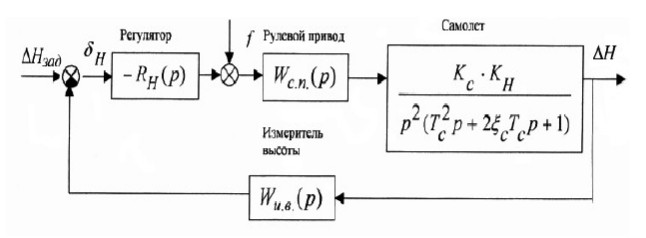
\includegraphics[width=\linewidth]{img/1.jpg}}
    \caption{Структурная схема системы стабилизации высоты}
    \label{fig:1}
\end{figure}
 
Устойчивость такого контура может быть обеспечина двумя путями: \\ 

1) введением внутренней стабилизирующей обратной связи по сигналу угла тангажа 
$\vartheta$, т.е. введением автопилота угла тангажа;\\

2) введением в закон управления $R_{H}(p)$ сигнал первой производной отклонения высоты для случая, если сервопривод имеет жёсткую обратную связь,
и ссумы сигналов первой и всторой производных от сигнала отклонения высоты для случая, 
когдасервопривод имеет скоростную или изодромную обратную связь.\\

На рис. \ref{fig:2} приведена структурная схема системы стабилизации высоты, содержащей автопилот угла тангажа.

\begin{figure}[H]
    \center{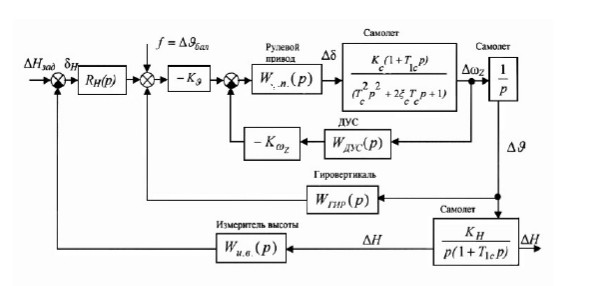
\includegraphics[width=\linewidth]{img/2.jpg}}
    \caption{Структурная схема системы стабилизации высоты}
    \label{fig:2}
\end{figure}

Основным приемуществом такой системы чвляется то, что устойчивость траекторного контура обеспечивается 
регулятором $R_H(p)=i_H$ за счёт сигнала угла тангажа, снимаемого с надёжного датчика -- гировертикали, практически лишённого запаздывания.
Система содержащая регулятор $R_H(p)=i_H$, называется статической системой т.к. этот регулятор не обеспечивает астатизм регулярования в отношении других возмущений. 


\begin{equation}
    \begin{cases}
        \Delta\dot{\alpha}=\Delta\omega_z-\bar{Y}^\alpha_a\Delta\alpha\\
        \Delta\dot{\omega_z} = \bar{M}^\alpha_z\Delta\alpha+\bar{M}^{\omega_z}_z\Delta\omega_z+\bar{M}^{\delta_B}_z\Delta\delta_B\\
        \Delta\dot{\vartheta} = \Delta\omega_z\\
        \Delta\dot{V_y}=V_0\bar{Y}^\alpha_a\Delta\alpha\\
        \Delta\dot{H}=\Delta V_y\\
        \Delta n_y=n^\alpha_y\Delta\alpha
    \end{cases}
    \label{eq:СДУ}
\end{equation}

Где система (\ref{eq:СДУ}) -- это система дифференциальных уравнений, используемая для маделирования
движения самолёта в короткопериодическом движении. 

\begin{equation}
    \begin{cases}
        \Delta\delta_B=K_{\omega_z}\Delta\omega_z+K_{\vartheta}(\Delta\vartheta-\Delta\vartheta_\text{зад}+f)\\
        \Delta\vartheta_{\text{зад}} = i_H(\Delta H_{\text{зад}}-\Delta H)+i_p\int_{0}^{t}(\Delta H_{\text{зад}}-\Delta H)dt
    \end{cases}
    \label{eq:заданные значения}
\end{equation}

\section{Исходные данные}

    \begin{table}[H]
        \centering
        \caption{Исходные данные}
        \label{tab:Исходные данные 1}
        \begin{tabular}{|c|c|}
        \hline
            $m_0$ & 25000 кг  \\ \hline
            $S$ & 50 м$^2$ \\ \hline
            $b_a$ & 5м  \\ \hline
            $J_z$ & 50000 кг м$^2$ \\ \hline
            $H$ & 1000 м  \\ \hline
            $M$ & 0.5  \\ \hline
        \end{tabular}
    \end{table}
                                
    \begin{table}[H]
        \centering
        \caption{Исходные данные}
        \label{tab:Исходные данные 2}
        \begin{tabular}{|c|c|}
            \hline
            $\bar{Y}_a^\alpha=a_{11},$ $1/c$ &  0.642  \\ \hline
            $\bar{M}_z^{\alpha}=a_{21}$, $1/c^2$ &   5.65 \\ \hline
            $\bar{M}_z^{\omega_z}=a_{22}$,$1/c$ &  0.468 \\ \hline
            $\bar{M}^{\delta_B}_z=b_2$ & 4.5  \\ \hline
            $V_0=a_{46}$,м$/c$ & 168 \\ \hline
            $n_y^\alpha=a_{51}$ &  11.0  \\ \hline
            $K_{\omega_z}, c$ & 0.4 \\ \hline
            $K_\vartheta$  & 0.5, 1, 2  \\ \hline
            $i_H$ рад/м & 0.000875 0.00175 0.002625 \\ \hline
            $i_p$ рад/м & 0.0000875 0.000175 0.0002625 \\ \hline
            $\hat{t}_{cp},c$ & 8 \\ \hline
            $\hat{\sigma}_{\Delta H}, \%$ & 30 \\ \hline
            $\hat{n}_{y_{max}},c$ & 1.2 \\ \hline
            $\hat{H}_{\text{ст}},$ м & 20 \\ \hline
            \end{tabular}
    \end{table}

\section{Лабораторная работа №1. Исследование статической системы стабилизации высоты полета.}
\subsection{Выполнение работы}
    \subsubsection{Ход работы}
    
    \begin{enumerate}
    \item На персональном компьютере установить задачу 1, после чего в цикле для
    каждой   пары   коэффициентов  заданных   в  табл.   1,
    определяются:\\
    а)	при отработке управляющего воздействия  = 100м:
        \begin{itemize}
            \item время срабатывания   
            \item максимальное значение высоты  
            \item максимальное значение перегрузки.
        \end{itemize}
    б)	при отработке постоянного возмущения $f=$ -0.035 рад:
        \begin{itemize}
            \item статическую ошибку регулирования .
        \end{itemize}
    
    Результаты расчетов оформить в виде таблица \ref{tab:Результаты расчётов}.

    
    \begin{table}[H]
        \caption{\label{tab:Результаты расчётов} Нестандартные болты для левой резьбы.}
        \begin{center}
            \begin{tabular}{|c|c|c|c|c|}
            \hline
            & \multicolumn{1}{|c|}{} & \multicolumn{3}{|c|}{$i_H,$ рад/м}  \\
            \cline{3-5}
            \raisebox{1.5ex}[0cm][0cm]{$K_{\vartheta}$} & \raisebox{1.5ex}[0cm][0cm]{Показатель}
            & 0.000875 & 0.00175 &0.002625\\
            \hline
            & $t_{cp}, c$ & 15.82 & 9.5 & 7.3\\ 
            \cline{2-5} 
            & $\Delta H_{max},$ м & 115.1 & 131.3 & 141.5\\ 
            \cline{2-5} 
            0.5& $\sigma_{\Delta H},$ \% & 15.1 & 31.3 & 41.7\\ 
            \cline{2-5} 
            & $\Delta n_{y_{max}}$ & 0.27 & 0.54 & 0.809\\ 
            \cline{2-5} 
            & $\Delta H_{\text{ст}},$ м & 40 & 20 & 13.3\\ 
            \hline
            & $t_{cp}, c$ & 15.4 & 8.25 & 6.2\\
            \cline{2-5} 
            & $\Delta H_{max},$ м & 106.2 & 120.3 & 130.5\\ 
            \cline{2-5} 
            1& $\sigma_{\Delta H},$ \% & 6.2 & 20.3 & 30.5\\ 
            \cline{2-5} 
            & $\Delta n_{y_{max}}$ & 0.441 & 0.88 & 1.317\\ 
            \cline{2-5} 
            & $\Delta H_{\text{ст}},$ м & 40 & 20 & 13.3\\
            \hline
            & $t_{cp}, c$ & 17.1 & 7.7 & 5.55\\
            \cline{2-5} 
            & $\Delta H_{max},$ м & 101.5 & 112.5 & 121.2\\ 
            \cline{2-5} 
            2& $\sigma_{\Delta H},$ \% & 1.5 & 12.5 & 21.2\\ 
            \cline{2-5} 
            & $\Delta n_{y_{max}}$ & 0.576 & 1.145 & 1.707\\ 
            \cline{2-5} 
            & $\Delta H_{\text{ст}},$ м & 40 & 20 & 13.3\\ 
            \hline
            \end{tabular}
        \end{center}
    \end{table}

    \item Построить по данным табл. \ref{tab:Результаты расчётов} графики следующих зависимостей:
    $$t_{cp}=f_1(K_{\vartheta},i_H);\sigma_{\Delta H}=f_2(K_{\vartheta},i_H)$$
    $$\Delta n_{y_{max}}=f_3(K_{\vartheta},i_H);\Delta H_{\text{ст}}=f_4(K_{\vartheta},i_H)$$
    Нанести   на   графики   прямые   линии,   соответствующие   максимально допустимым величинам показателей качества переходных процессов  $t_{cp}$. 

    $\hat{\sigma}_{\Delta H}$;$\Delta n_{y_{max}}$;$\Delta \hat{H}_{\text{ст}}$(смотри табл. \ref{tab:Исходные данные 2})
    
    \begin{figure}[H]     % Графики к пункту 2
        \center{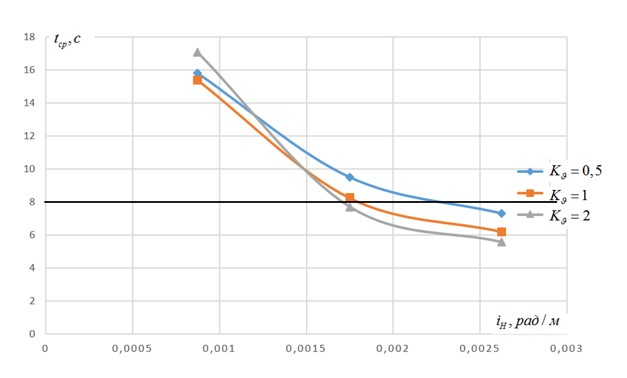
\includegraphics[width=\linewidth]{img/3.jpg}}
        \caption{Время срабатывания $t_{cp},$ c}
        \label{fig:Время срабатывания}
    \end{figure}
    
    \begin{figure}[H]
        \center{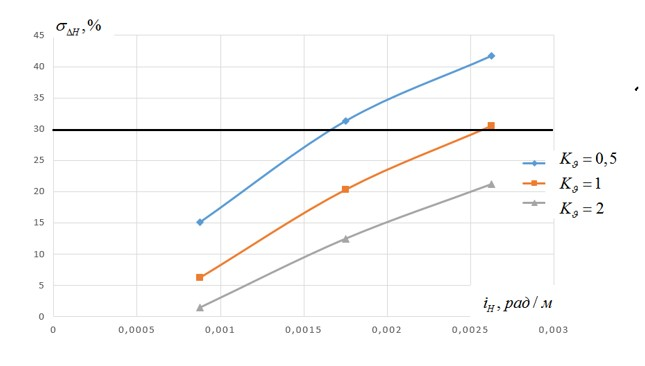
\includegraphics[width=\linewidth]{img/4.jpg}}
        \caption{Относительное перерегулирование $\sigma_{\Delta H},$ \%}
        \label{fig:Относительное перерегулирование}
    \end{figure}
    
    \begin{figure}[H]
        \center{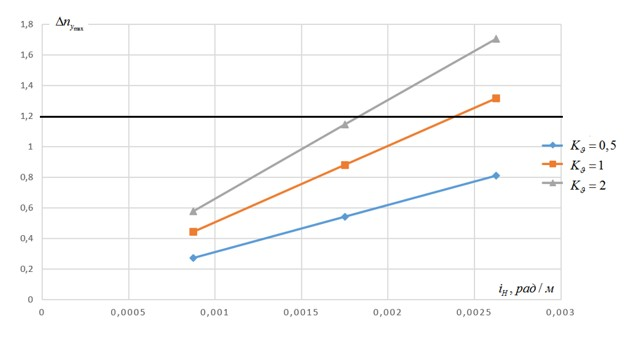
\includegraphics[width=\linewidth]{img/5.jpg}}
        \caption{Максимальное значение нормальной перегрузки $\Delta n_{y_{max}}$}
        \label{fig:Максимальное значение нормальной перегрузки}
    \end{figure}
    
    \begin{figure}[H]
        \center{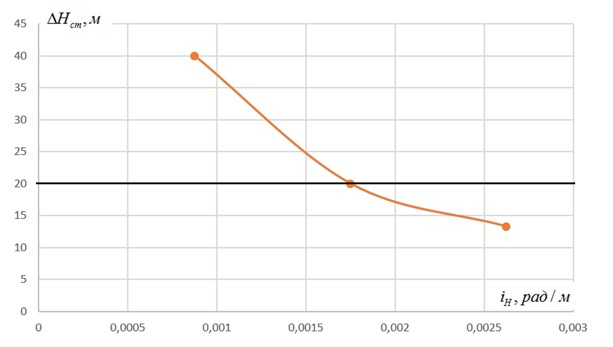
\includegraphics[width=\linewidth]{img/6.jpg}}
        \caption{Статистическая ошибка по высоте $\Delta H_{\text{ст}},$ м}
        \label{fig:Статистическая ошибка по высоте}
    \end{figure}


    \item Построить, используя зависимости п. 2, допустимую область изменения коэффициентов усиления $K_{\vartheta}=f(i_H)$ из условия \\ $t_{cp} \leq \hat{t}_{cp}$; $\sigma_{\Delta H} \leq \hat{\sigma}_{\Delta H}$;
    $\Delta n_{y_{max}} \leq \Delta \hat{n}_{y{max}}$; $\Delta H_{\text{ст}} \leq \Delta \hat{H}_{\text{ст}}$  

    % Графики пункта 3
    \begin{figure}[H]
        \center{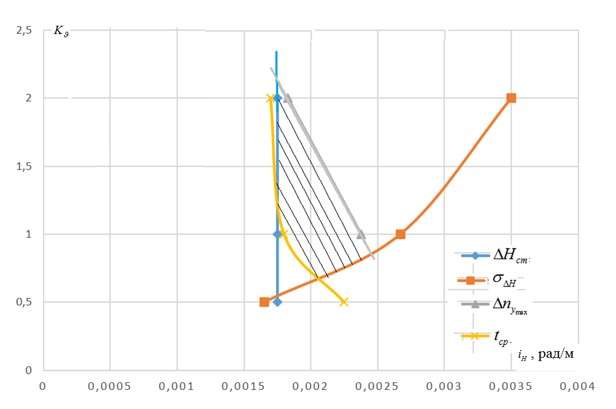
\includegraphics[width=\linewidth]{img/7.jpg}}
        \caption{Область изменения коэффициента усиления}
        \label{fig:Область изменения коэффициента усиления}
    \end{figure}

    \end{enumerate}
    
    \subsubsection{Переходные процессы}

    \begin{figure}[H]
        \center{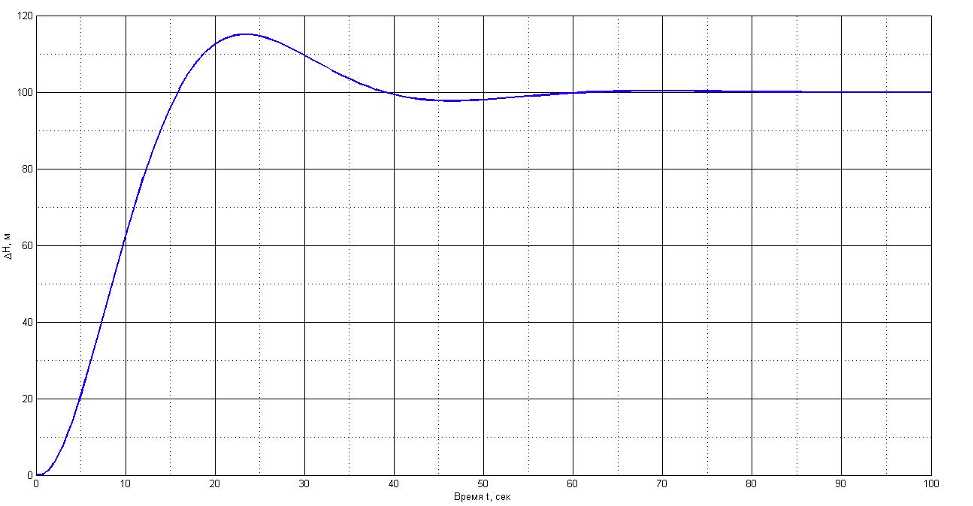
\includegraphics[width=\linewidth]{img/8.png}}
        \caption{График ппереходного процесса при $K_{\vartheta}=0.5, i_H=0,000875$ [рад/м], $f=0$}
        \label{fig:Переходный процесс 1}
    \end{figure}

    \begin{figure}[H]
        \center{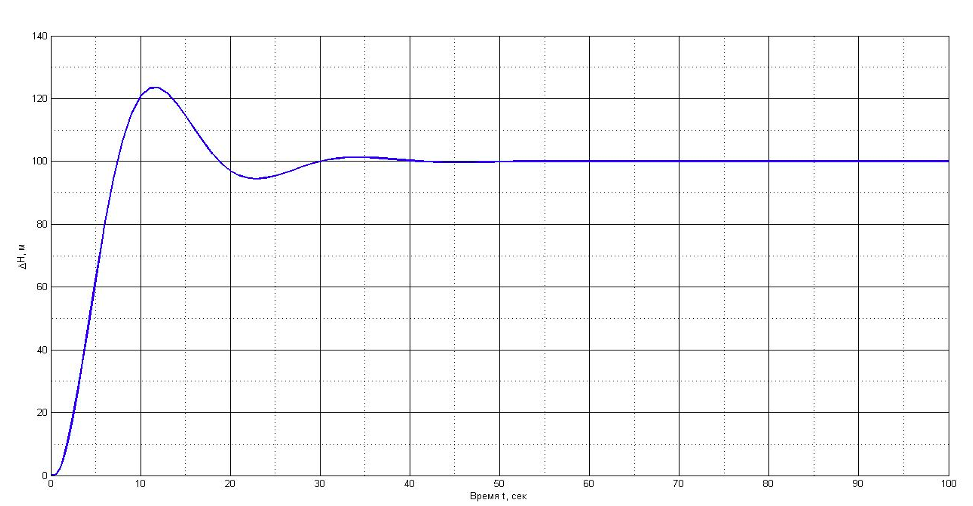
\includegraphics[width=\linewidth]{img/9.png}}
        \caption{График ппереходного процесса при $K_{\vartheta}=1, i_H=0,002$[рад/м], $f=0$}
        \label{fig:Переходный процесс 2}
    \end{figure}

    \subsubsection{Выводы}
    \begin{enumerate}
        \item Статическая ошибка, возникающая при наличии возмущений, уменьшается с увеличением коэффициентов стабилизации.
        \item При увеличении $K_{\vartheta}$  и $i_H$, рад/м время срабатывания системы уменьшается.
        \item При увеличении коэффициентов $K_{\vartheta}$  и $i_H$ $\Delta n_{y_{max}}$ возрастает. 
        \item Относительное перерегулирование при увеличении коэффициента $K_{\vartheta}$ уменьшается, а при увеличении $i_H$ увеличивается.
    \end{enumerate}

\section{Лабораторная работа №2. Исследование астатической системы стабилизации высоты полета.}
    \subsection{Выполнение работы}
        \subsubsection{Ход работы}
            	\begin{enumerate}
		            \item Установить на персональном компьютере задачу 2, после чего выставить
                        значения коэффициентов $K_{\vartheta}$, $i_H$ соответствующие центру допустимой
                        области изменения коэффициентов усиления $K_{\vartheta}=f(H)$. Далее в цикле для
                        каждого значения коэффициента  $i_p$ (см. табл. \ref{tab:Исходные данные 2}) определяются:
                            \begin{itemize}
                                \item[a)] при отработке управляющего воздействия $\Delta H_{зад}$ = 100м:
                                        максимальное значение высоты ;
                                \item[б)] при отработке постоянного возмущения  $f=-0.035$ рад:
                                время регулирования   (время, по истечению которого переходный процесс  входит в 5\%-ную трубку установившегося значения
                                относительно ).
                            \end{itemize}
                            Результаты расчетов приведены в виде таблицы \ref{tab:Таблица с результатами лаба2}.
                            
                            \begin{table}[H]
                                \centering
                                \caption{Результаты расчётов при $K_{\vartheta}=2, i_H=0.00175$, рад/с}
                                \begin{tabular}{|c|c|c|c|}
                                \hline
                                    $i_p$рад/м/с & 0.0000875 & 0.000175 &0.00035\\ \hline
                                    $t_{\text{рег}}, c$ & 42 & 37 &86\\ \hline
                                    $\Delta H_{max},$ м &  138.7  & 154.6 & 180.1 \\ \hline
                                    $\sigma_{\Delta H}, \%$  & 38.7  & 154.6  &  80.1 \\ \hline
                                \end{tabular}
                                \label{tab:Таблица с результатами лаба2}
                            \end{table}
                            
                            % \begin{table}[H]   %%Таблица с запасным вариантом
                            %     \centering
                            %     \begin{tabular}{|c|c|c|c|}
                            %     \hline
                            %         $i_p$рад/м/с & 0.0000875 & 0.000175 &0.00035\\ \hline
                            %         $t_{\text{рег}}, c$ & 40 & 27 &66\\ \hline
                            %         $\Delta H_{max},$ м &  131.8  & 148.2 & 173.4 \\ \hline
                            %         $\sigma_{\Delta H}, \%$  & 31.7  & 48.2 &  73.4 \\ \hline
                            %     \end{tabular}
                            %     \caption{Результаты расчётов при $K_{\vartheta}=2,         i_H=0.00175$, рад/с}
                            %     \label{tab:Таблица с результатами лаба2}
                            % \end{table}
                            
                        \item Построить по данным табл. \ref{tab:Таблица с результатами лаба2} графики следующих зависимостей:
                            \begin{itemize}
                                \item  $\sigma_{H}(i_p)$ при отработке управляющего воздействия $\Delta H_{\text{зад}}$;
                                \item  $t_{\text{рег}}(i_p)$  при отработке возмущения
                            \end{itemize}
                            \begin{figure}[H]
                                \centering
                                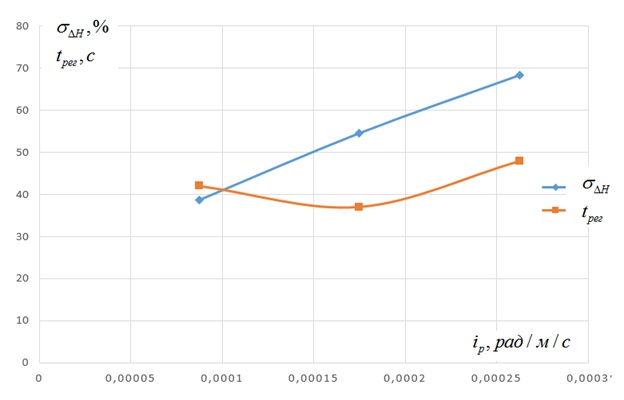
\includegraphics[widht=\linewidth]{img/10.jpg}
                                \caption{График зависимостей $\sigma_{H}(i_p)$ и $t_{\text{рег}}(i_p)$ }
                                \label{fig:my_label}
                            \end{figure}
                            
                            % \begin{figure}[H]
                            %     \centering
                            %     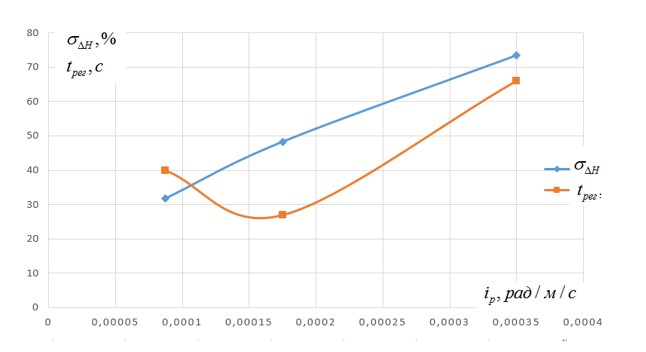
\includegraphics[widht=\linewidth]{img/11.jpg}
                            %     \caption{График зависимостей $\sigma_{H}(i_p)$ и $t_{\text{рег}}(i_p)$ }
                            %     \label{fig:my_label}
                            % \end{figure}
                            
                \end{enumerate}
                \subsubsection{Выводы}
                \begin{enumerate}
                    \item При увеличении $i_p$ относительное перерегулирование  возрастает.
                    \item Зависимость $t_{\text{рег}}(i_p)$ имеет минимум $i^*_p$  до которого время регулирования уменьшается, а далее возрастает. В данной работе $i^*_p=0.00015$ 
                \end{enumerate}
\end{document} 
